\documentclass[fleqn]{beamer}

\usepackage[british]{babel}
\usepackage{graphicx,ru,url}
\usepackage{amsmath}
% Use Times for math font and text font.
\RequirePackage[T1]{fontenc}
%\RequirePackage{txfonts}
% bold math must be loaded after Times font
\usepackage{bm}
\usepackage{booktabs} % nice rules (thick lines) for tables
\usepackage{microtype} % improves typography for PDF
\usepackage{xcolor} % Allows colors in fonts
\usepackage{tikz} % Allows creation of tikz pictures
\usepackage{verbatim}
\usetikzlibrary{arrows,shapes,snakes}
\usepackage{hyperref}
\usepackage{algorithmic,algorithm}
\usepackage{verbatim}
\usepackage{braket}
\usepackage{longtable}
\usepackage[parfill]{parskip}
\usepackage{standalone}
\usepackage[backend=bibtex, style=authortitle-icomp,maxnames=99]{biblatex}
\addbibresource{bibliography.bib}

\newcommand{\SN}{S$_N$}
\renewcommand{\vec}[1]{\bm{#1}} %vector is bold italic
\newcommand{\vd}{\bm{\cdot}} % slightly bold vector dot
\newcommand{\grad}{\vec{\nabla}} % gradient
\newcommand{\ud}{\mathop{}\!\mathrm{d}} % upright derivative symbol
\newcommand{\oper}[1]{\mathcal{#1}}
\providecommand{\e}[1]{\ensuremath{\times 10^{#1}}}
\newcommand{\CHAPTER}[1]{Chapter~\ref{#1}} 
\newcommand{\EQ}[1]{Eq.~(\ref{#1})}               %-- Eq. (refeq)
\newcommand{\EQUATION}[1]{Equation~(\ref{#1})}    %-- Equation (refeq)
\newcommand{\FIG}[1]{Fig.~\ref{#1}}               %-- Fig. refig
\newcommand{\FIGURE}[1]{Figure~\ref{#1}} 
\newcommand{\TAB}[1]{Table~\ref{#1}}              %-- Table tablref
\newcommand{\EQS}[2]{Eqs.~(\ref{#1})--(\ref{#2})}            %-- Eqs. (refeqs)
\newcommand{\EQUATIONS}[2]{Equations~(\ref{#1})--(\ref{#2})}   %-- Eqs. (refeqs)
\newcommand{\EQSTWO}[2]{Eqs.~(\ref{#1})~and~(\ref{#2})}     %-- Eqs. (refeqs)
\newcommand{\EQUATIONSTWO}[2]{Equations~(\ref{#1})~and~(\ref{#2})} 

% The title of the presentation:
%  - first a short version which is visible at the bottom of each slide;
%  - second the full title shown on the title slide;
\title[DMD-PM]{Acceleration of the Power and Related Methods with Dynamic Mode Decomposition}

% Optional: a subtitle to be displayed on the title slide
%\subtitle{Show where you're from}

% The author(s) of the presentation:
%  - again first a short version to be displayed at the bottom;
%  - next the full list of authors, which may include contact information;
\author[Leidong Xu]{Leidong Xu\\ Advisor: Dr. Jeremy Roberts}

% The institute:
%  - to start the name of the university as displayed on the top of each slide
%    this can be adjusted such that you can also create a Dutch version
%  - next the institute information as displayed on the title slide
\institute[Kansas State University]{
    Alan Levin Department of Mechanical and Nuclear Engineering\\
    Carl R. Ice College of Engineering \\
    Kansas State University}

% Add a date and possibly the name of the event to the slides
%  - again first a short version to be shown at the bottom of each slide
%  - second the full date and event name for the title slide
\date[Master's Defense]{
    Master's Defense \\
    November.8.2019}

\begin{document}
    % These two commands allow bonus slides at the end
    % The bonus slides will not be numbered
    \newcommand{\beginbackup}{
        \newcounter{framenumbervorappendix}
        \setcounter{framenumbervorappendix}{\value{framenumber}}
    }
    \newcommand{\backupend}{
        \addtocounter{framenumbervorappendix}{-\value{framenumber}}
        \addtocounter{framenumber}{\value{framenumbervorappendix}} 
    }
    
    \begin{frame}
        \titlepage
    \end{frame}
    
    \begin{frame}
        \frametitle{Outline}
        \begin{block}{Presentation Outline}
            \begin{itemize}
                \item K-eigenvalue Problem
                \item DMD-PM(n)
                \item DMD-FPM(n)
                \item Conclusion and Future Work
            \end{itemize}
        \end{block}
    \end{frame}

%%%%%%%%%%%%%%%%%%%%%%%%%%%%%%%% introduction    
\section{Neutron Transport}
\begin{frame}
\frametitle{Neutron Transport}
\begin{block}{Multigroup Neutron Transport Equation}
\vspace*{-\baselineskip}\setlength\belowdisplayshortskip{0pt}
\begin{equation*}
\begin{split}
  \bm{\hat{\Omega}} & \cdot \nabla \psi_g(\vec{r},\bm{\hat{\Omega}}) +
    \Sigma_{t g}(\vec{r}) \psi_{g}(\vec{r},\bm{\hat{\Omega}}) = \\
   & \frac{1}{4\pi} \sum\limits^{N_g}_{g'=1} \Sigma_{s g g'}(\vec{r}) \phi_{g'}(\vec{r}) +
    \frac{\chi_g}{4\pi k} \sum\limits^{N_g}_{g'=1} \nu\Sigma_{fg'}(\vec{r}) \phi_{g'}(\vec{r}) 
\end{split}
\label{eq:transport}
\end{equation*}
\end{block}
\begin{block}{K-eigenvalue Problem}
\begin{enumerate}
  \item Steady-state solution
  \item Criticality analysis
\end{enumerate}
\end{block}
\end{frame}    

\begin{frame}
\frametitle{Generic Eigenvalue Problem\footnotemark}
\begin{block}{Operator Notation}
\vspace*{-\baselineskip}\setlength\belowdisplayshortskip{0pt}
\begin{equation*}
  \mathbf{D} \psi =  \mathbf{DL}^{-1}\mathbf{MS}\phi + \frac{1}{k} \mathbf{DL^{-1}MF} \phi  
 \label{eq:operatortrans}
\end{equation*}
\begin{equation*}
  \mathbf{(I - DL^{-1}MS)} \mathbf{\phi} = \frac{1}{k} \mathbf{DL^{-1}MF} \mathbf{\phi}  
 \label{eq:keig}
\end{equation*}
\begin{equation*}
 \mathbf{Ax} = \frac{1}{k} \mathbf{Bx}  
 \label{eq:Axb}
\end{equation*}
$\mathbf{M}$ is the moment-to-discrete operator\\
$\mathbf{D}$ is the discrete-to-moment operator\\
$\mathbf{L}$ is the loss operator\\
$\mathbf{F}$ is the fission operator\\
$\mathbf{S}$ is the scattering operator\\
k is ratio of neutron gains to losses.
\end{block}
\footnotetext{\cite{roberts_multigroup_2014}}
\end{frame}    

%%%%%%%%%%%%%%%%%%%%% Power Method
\subsection{Power Method}
\begin{frame}
\frametitle{Power Method}
\begin{block}{Algorithm}
\begin{enumerate}
  \item Initialize $\lambda^{(0)}_0$ and $\mathbf{x}^{(0)}_0$ 
  \item Set $\mathbf{x}^{(i)}_0=\mathbf{A}\mathbf{x}^{(i-1)}_0$
  \item Update $\lambda_{i} = ||\mathbf{x}^{(i)}_0||$ and normalize $\mathbf{x}^{(i)} =\frac{\mathbf{x}^{i}}{||\mathbf{x}^{i}||}$
  \item Repeat steps 2 and 3 
\end{enumerate}
\end{block}
\end{frame}    

\subsection{Dynamic Mode Decomposition}
%%%%%%%%%%%%%%%%%%%%% DMD
\begin{frame}
\frametitle {Dynamic Mode Decomposition}
A sequential dataset ($\mathbf{X} \subseteq \mathbb{R}^{n\times m}$) spaced by $\Delta t$.\footnotemark
\begin{figure}[!htb]
\centering
\includegraphics[scale=0.17]{figures/snapshot.jpg}
\label{fig:data_matrix}
\end{figure} 
\begin{block}{}
\small{\textbf{Assumption}}: 
$
\mathbf{X_1} \approx  \tikz[baseline]{\node[draw=purple,anchor=base,
circle,inner xsep=-2pt,inner ysep=3pt] {$\mathbf{A}$}} \mathbf{X_0}
$
\end{block}
\footnotetext{\cite{schmid_dynamic_2010},\cite{schmid_applications_2011}} 
\end{frame}

\begin{frame}
\frametitle{Dynamic Mode Decomposition}
\begin{block}{Algorithm}
\begin{enumerate}
\item SVD decomposition of $ \mathbf{X_0} = \mathbf{U_r} \boldsymbol{\Sigma_r} \mathbf{V_r^{*}}$
\pause
\item Compute $\mathbf{\tilde{A}}=\mathbf{U_r^{*}AU_r}=\mathbf{U_r^{*}X_1}\mathbf{V_r}\boldsymbol{\Sigma}_{\mathbf{r}}^{-1}$
\pause
\item Compute the eigendecomposition $\mathbf{\tilde{A} \tilde{W}}=\boldsymbol{\Lambda}\mathbf{\tilde{W}}$
\pause
\item Calculate the DMD modes as ${\boldsymbol{\Phi}}={\mathbf{X_1V_r}}\boldsymbol{\Sigma}_\mathbf{r}^{-1}{\mathbf{\tilde{W}}}$
\pause
\item Predict the response by $\vec{x}^{DMD}(t) \approx \sum_{i=1}^{r} \vec{\phi}_i e^{\omega_it} b_i = \boldsymbol{\Phi}{\mathbf{diag}}(e^{\vec{\omega}t})\boldsymbol{\Phi}^{\dag} \mathbf{x}_{0}$
\end{enumerate}
\end{block}
\end{frame}  

%%%%%%%%%%%%%%%%%%%%% Objective
\begin{frame}
\begin{block}{Objective}
To estimate accurate fundamental eigenmodes using DMD to accelerate the power method and other, related methods.
\begin{itemize}
\item Less computational cost
\item Fast convergence
\end{itemize}
\end{block}
\end{frame}

%%%%%%%%%%%%%%%%%%%%% IAEA 
\begin{frame}
\frametitle{2D 2-group IAEA  Diffusion Benchmark\footnotemark}
\begin{figure}
\label{fig:IAEA}
\centering
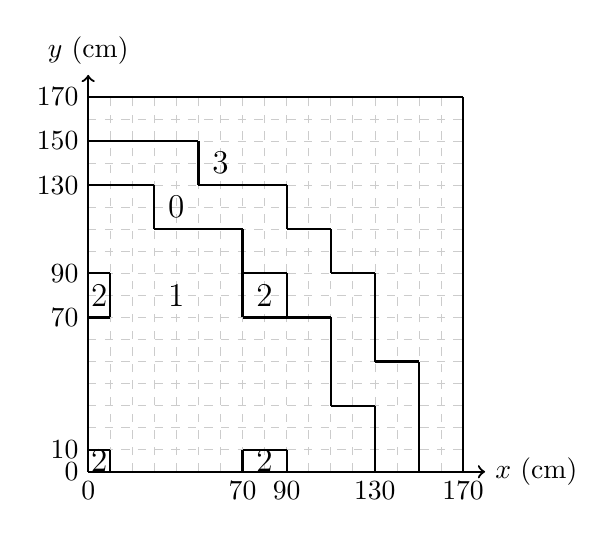
\begin{tikzpicture}[scale=.28]
\begin{scope}<->;
% GRID
 \draw[step=1.0,gray,very thin, dashed,opacity=0.4] (0.0,0.0) grid (17.0, 17.0); 
  
% AXES
  \draw[black, thick, ->] (0, 0) -- (18,  0) node[right] {$x$ (cm)};
  \draw[black, thick, ->] (0, 0) -- ( 0, 18) node[above] {$y$ (cm)};

% Material 3 regions
  \draw[black, thick] (  0.0, 17.0) -- (17.0, 17.0);
  \draw[black, thick] (  17.0, 17.0) -- (17.0, 0.0);  
  \node[font=\large] at (6.0, 14.0) {3};

% Material 0 regions
  \draw[black, thick] (  0.0, 15.0) -- (5.0, 15.0);
  \draw[black, thick] (  5.0, 15.0) -- (5.0, 13.0);  
  \draw[black, thick] (  5.0, 13.0) -- (9.0, 13.0);
  \draw[black, thick] (  9.0, 13.0) -- (9.0, 11.0);
  \draw[black, thick] (  9.0, 11.0) -- (11.0, 11.0); 
  \draw[black, thick] (  11.0, 11.0) -- (11.0, 9.0); 
  \draw[black, thick] (  11.0, 9.0) -- (13.0, 9.0); 
  \draw[black, thick] (  13.0, 9.0) -- (13.0, 5.0);
  \draw[black, thick] (  15.0, 5.0) -- (13.0, 5.0);
  \draw[black, thick] (  15.0, 5.0) -- (15.0, 0.0);
  \node[font=\large] at (4.0, 12.0) {0};

% Material 1 regions
  \draw[black, thick] (  0.0, 13.0) -- (3.0, 13.0);
  \draw[black, thick] (  3.0, 13.0) -- (3.0, 11.0);  
  \draw[black, thick] (  3.0, 11.0) -- (7.0, 11.0);
  \draw[black, thick] (  7.0, 11.0) -- (7.0, 7.0);
  \draw[black, thick] (  7.0, 7.0) -- (11.0, 7.0); 
  \draw[black, thick] (  11.0, 7.0) -- (11.0, 3.0);  
  \draw[black, thick] (  11.0, 3.0) -- (13.0, 3.0);  
  \draw[black, thick] (  13.0, 3.0) -- (13.0, 0.0);  
  \node[font=\large] at (4.0, 8.0) {1};

% Material 2 regions
  \draw[black, thick] (  0.0, 0.0) -- (0.0, 1.0);
  \draw[black, thick] (  1.0, 1.0) -- (1.0, 0.0);  
  \draw[black, thick] (  0.0, 1.0) -- (1.0, 1.0);
  \node[font=\large] at (0.5, 0.5) {2};  
  
  \draw[black, thick] (  0.0, 7.0) -- (1.0, 7.0); 
  \draw[black, thick] (  1.0, 7.0) -- (1.0, 9.0);  
  \draw[black, thick] (  1.0, 9.0) -- (0.0, 9.0);  
  \node[font=\large] at (0.5, 8.0) {2};  
  
  
  \draw[black, thick] (  7.0, 7.0) -- (9.0, 7.0);  
  \draw[black, thick] (  9.0, 7.0) -- (9.0, 9.0);  
  \draw[black, thick] (  9.0, 9.0) -- (7.0, 9.0);  
  \node[font=\large] at (8.0, 8.0) {2};

  \draw[black, thick] (  7.0, 0.0) -- (9.0, 0.0);
  \draw[black, thick] (  9.0, 0.0) -- (9.0, 1.0);
  \draw[black, thick] (  9.0, 1.0) -- (7.0, 1.0);
  \draw[black, thick] (  7.0, 1.0) -- (7.0, 0.0);
  \node[font=\large] at (8.0, 0.5) {2}; 
 
% ticks
  \foreach \x/\xtext in {0, 70, 90, 130, 170}
      \draw[black,xshift=0.1*\x cm] (0,.3) -- (0,0) node[below] {$\xtext$};
  \foreach \y/\ytext in {0, 10, 70, 90, 130, 150, 170}
      \draw[black,yshift=0.1*\y cm] (.3,0) -- (0,0) node[left] {$\ytext$};

\end{scope}
\end{tikzpicture}
\label{fig:iaea2d}
\end{figure}
\footnotetext{\cite{center1977benchmark}}
\end{frame}

\begin{frame}
\frametitle{Skip Ahead}
\begin{figure}
\centering
\includegraphics[width = \textwidth]{figures/skipahead.pdf}
\end{figure}
\end{frame}

\begin{frame}
\frametitle{DMD-PM(n)}
\begin{block}{Modified DMD Algorithm for eigenpair}
\vspace*{-\baselineskip}\setlength\belowdisplayshortskip{0pt}
\begin{equation*}
\label{eq:full_prediction}
\mathbf{x}(t) \approx \sum^{m}_{i=1} \mathbf{\phi}_i e^{\omega_i t} b_i = \boldsymbol{\Phi} e^{\bm{\Omega}t} \mathbf{b} \, 
\end{equation*}
An extrapolated guess with just the dominant mode \footnotemark
\begin{equation*}
\mathbf{\phi}_i e^{\omega_i t} b_i \approx 0 , i  > 1, t \rightarrow \infty
\end{equation*}
\begin{equation*}
\label{eq:f_mode}
\vec{x}^{DMD}(\infty) \approx \vec{\phi}_0 b_0 
\end{equation*}
\end{block}
\footnotetext{\cite{roberts2019acceleration}}
\end{frame} 

%%%%%%%%%%%%%%%%%%%%% DMD-PM
\section{DMD-PM(n)}
\begin{frame}
\frametitle{DMD-PM(n)}
\begin{block}{Algorithm}
\begin{enumerate}
 \item Guess $\mathbf{x}^{(0)}$ and normalize.
 \item Perform $n$ power iterations to produce $\mathbf{X}_0$ and $\mathbf{X}_1$
 \item Compute the $r$th DMD modes 
 \item Estimate $\mathbf{x}^{(\infty)}=\mathbf{x}(\infty)$
 \item Set $\mathbf{x}^{(0)} = \Re(\mathbf{x}(\infty)) / ||\mathbf{x}(\infty)||$.  
 \item Repeat Steps 1 through 5 until converged.
\end{enumerate}
\end{block}
\end{frame}  

\begin{frame}
\frametitle{IAEA 2-D diffusion}
\begin{figure}
\centering
\includegraphics[width =\textwidth]{figures/dmdpi_semilog.pdf}
\end{figure}
\end{frame}

\begin{frame}
\frametitle{BCSSTK29}
\begin{columns}[c]
\begin{column}{.5\textwidth}
\begin{figure}
\includegraphics[width=\textwidth]{figures/bcsstk29_sm.png}
\caption{BCS Structural Engineering Matrix}
\end{figure}
\end{column}
\begin{column}{.5\textwidth}
\begin{itemize}
\item The buckling model of a Boeing 767 rear pressure bulkhead. 
\item Matrix dimension: 13992 x 13992.
\item Only non-zero 316740 entries.
\end{itemize}
\end{column}
\end{columns}
\end{frame}

\begin{frame}
\frametitle{BCSSTK29}
\begin{figure}
\centering
\includegraphics[width = 0.9\textwidth]{figures/boeing_error.png}
\caption{The error in the predicted eigenmode}
\end{figure}
\end{frame}

%%%%%%%%%%%%%%%%%%%%% Flattened Power Method
\section{DMD-FPM(n)}

\begin{frame}
\frametitle{Power Method}
Large computation cost on step 2
\begin{block}{Algorithm}
\begin{enumerate}
  \item Initialize $\lambda^{(0)}_0$ and $\mathbf{x}^{(0)}_0$ 
  \item Set $\mathbf{x}^{(i)}_0=\mathbf{A}\mathbf{x}^{(i-1)}_0$
  \item Update $\lambda_{i} = ||\mathbf{x}^{(i)}_0||$ and normalize $\mathbf{x}^{(i)} =\frac{\mathbf{x}^{i}}{||\mathbf{x}^{i}||}$
  \item Repeat steps 2 and 3 
\end{enumerate}
\end{block}
\end{frame}    

\begin{frame}
\frametitle{Flattened Power Method}
\begin{block}{Complete solution of the inhomogeneous equation}
\vspace*{-\baselineskip}\setlength\belowdisplayshortskip{0pt}
\begin{equation*}
    \mathbf{Tx}^{i} = \mathbf{Fx}^{i-1}
\end{equation*}
\end{block}
\begin{block}{Flattened Operator\footnotemark}
\vspace*{-\baselineskip}\setlength\belowdisplayshortskip{0pt}
\begin{equation*}
 \mathbf{x}^{(i)} =  \mathbf{DL^{-1}M} (\mathbf{S} + \frac{1}{k} \mathbf{F})\mathbf{x}^{(i-1)}   
 \label{eq:flatten}
\end{equation*}
\end{block}
\footnotetext{\cite{gill_newtons_2011}}
\end{frame}  

\begin{frame}
\frametitle{DMD-FPM(n)}
How to match the DMD predictions?
\begin{block}{Aitken Extrapolation\footnotemark }
\vspace*{-\baselineskip}\setlength\belowdisplayshortskip{0pt}
\begin{equation*}
k_{aitken} = k_{i-2} - \frac{(k_{i-1}-k_{i-2})^2}{(k_i - 2k_{i-1} + k_{i-2})}
\end{equation*}
\end{block}
\footnotetext{\cite{aitken_1927}}
\end{frame}

%%%%%%%%%%%%%%%%%%%%% DMD-FPM
\begin{frame}
\frametitle{DMD-FPM (n)}
How do we estimate the corresponding eigenvalue?
\begin{block}{Algorithm\footnotemark}
\begin{enumerate}
 \item Assume $k_{(0)}$, $\mathbf{x}_{(0)}$ and normalize
 \item Perform $n$ flattened operator to produce $\mathbf{X}_0$ and $\mathbf{X}_1$
 \item Compute the DMD modes
 \item Apply equation $\mathbf{x}_{0}=\frac{b_0 \vec{\phi}^{}_0}{ ||b_0 \vec{\phi}^{}_0||}$ to estimate $\mathbf{x}^{(\infty)}=\mathbf{x}(\infty)$
 \item Update $k_{(0)}$ by Aitken extrapolation
 \item Repeat Steps 1 through 5 until converged
\end{enumerate}
\end{block}
\footnotetext{\cite{xu_acceleration}}
\end{frame}   

\begin{frame}
\frametitle{Configuration of 1D Boiling Water Reactor \footnotemark }
\begin{figure}
\centering
\begin{minipage}[c]{\textwidth}
    \centering
    \includestandalone[mode=buildnew, width=0.85\linewidth]{figures/core1}
\end{minipage}
\begin{minipage}[c]{\textwidth}
    \centering
    \includestandalone[mode=buildnew, width=0.3\linewidth]{figures/assemblies}
\end{minipage}
\begin{minipage}[c]{\textwidth}
    \centering
    \includestandalone[mode=buildnew, width=0.7\linewidth]{figures/core_materials}
\end{minipage}
\label{fig:BWRconfig}
\end{figure}
\footnotetext{\cite{rahnema_generalized_2008}}
\begin{block}{}
\begin{itemize}
    \item fuel region - 18 mesh cells
    \item moderator - 6 mesh cells
\end{itemize}
\end{block}
\end{frame}

\begin{frame}
\frametitle{1D Boiling Water Reactor Test}
\begin{figure}
\centering
\includegraphics[scale=0.5]{figures/dmd_ospi_semilog_1d.pdf}
\end{figure}
\end{frame}

\begin{frame}
\frametitle{Configuration for the C5G7 benchmark\footnotemark}
\begin{figure}
    \centering
    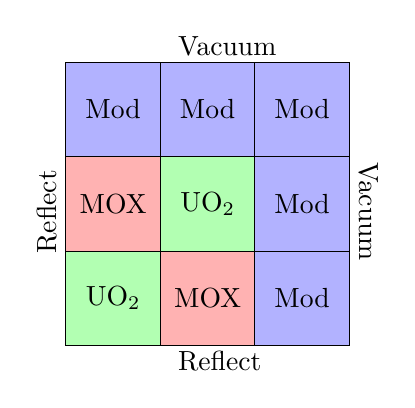
\begin{tikzpicture}[scale=0.4, every node/.style={scale=1}]
        \filldraw[xshift=6 cm, yshift=0 cm, fill=blue!30!white, draw=black] 
        (0, 0) rectangle (3,3) node[pos=.5] {Mod};
        \filldraw[xshift=6 cm, yshift=3 cm, fill=blue!30!white, draw=black] 
        (0, 0) rectangle (3,3) node[pos=.5] {Mod};
        \filldraw[xshift=6 cm, yshift=6 cm, fill=blue!30!white, draw=black] 
        (0, 0) rectangle (3,3) node[pos=.5] {Mod};
        \filldraw[xshift=3 cm, yshift=6 cm, fill=blue!30!white, draw=black] 
        (0, 0) rectangle (3,3) node[pos=.5] {Mod};
        \filldraw[xshift=0 cm, yshift=6 cm, fill=blue!30!white, draw=black] 
        (0, 0) rectangle (3,3) node[pos=.5] {Mod};
        \filldraw[xshift=0 cm, yshift=0 cm, fill=green!30!white, draw=black] 
        (0, 0) rectangle (3,3) node[pos=.5] {UO$_2$};
        \filldraw[xshift=3 cm, yshift=3 cm, fill=green!30!white, draw=black] 
        (0, 0) rectangle (3,3) node[pos=.5] {UO$_2$};
        \filldraw[xshift=3 cm, yshift=0 cm, fill=red!30!white, draw=black] 
        (0, 0) rectangle (3,3) node[pos=.5] {MOX};
        \filldraw[xshift=0 cm, yshift=3 cm, fill=red!30!white, draw=black] 
        (0, 0) rectangle (3,3) node[pos=.5] {MOX};
        \draw[xshift=9cm,yshift=4.25cm] node[right] 
        {\rotatebox{-90}{Vacuum}};
        \draw[yshift=4.25cm] node[left] {\rotatebox{90}{Reflect}};
        \draw[xshift=3.25cm,yshift=9.5cm] node[right] {{Vacuum}};
        \draw[xshift=3.25cm, yshift=-.5cm] node[right] {{Reflect}};
    \end{tikzpicture}
    \label{fig:C5G7_config}
\end{figure}
\footnotetext{\cite{oecd_nuclear_energy_agency_benchmark_2003}}
\end{frame}

\begin{frame}
\frametitle{Pin Assembly}
\begin{columns}[c]
\begin{column}{.45\textwidth}
\begin{figure}
    \centering
    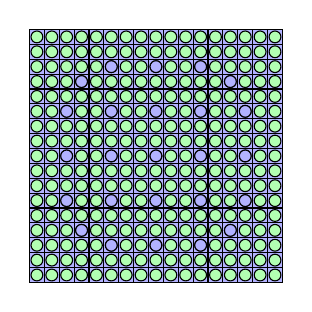
\begin{tikzpicture}[scale=0.15, every node/.style={scale=1}]
        \foreach \x in {0,1.26,...,20.16}
        \foreach \y in {0,1.26,...,20.16}
        \filldraw[xshift=\x cm, yshift=\y cm, fill=blue!30!white, 
        draw=black] (0, 0) rectangle (1.26,1.26) node[pos=.5] {};
        \foreach \x in {0,1.26,...,20.16}
        \foreach \y in {0,1.26,...,20.16}
        \filldraw[xshift=\x cm, yshift=\y cm, fill=green!30!white, 
        draw=black] (.63,.63) circle (.5) node[pos=.5] {};
        \foreach \x in {5*1.26, 8*1.26, 11*1.26}
        \foreach \y in {2*1.26, 14*1.26}
        \filldraw[xshift=\x cm, yshift=\y cm, fill=blue!30!white, 
        draw=black] (.63,.63) circle (.5) node[pos=.5] {};
        \foreach \x in {3*1.26, 13*1.26}
        \foreach \y in {3*1.26, 13*1.26}
        \filldraw[xshift=\x cm, yshift=\y cm, fill=blue!30!white, 
        draw=black] (.63,.63) circle (.5) node[pos=.5] {};
        \foreach \x in {2*1.26, 5*1.26, 8*1.26, 11*1.26, 14*1.26}
        \foreach \y in {5*1.26, 8*1.26, 11*1.26}
        \filldraw[xshift=\x cm, yshift=\y cm, fill=blue!30!white, 
        draw=black] (.63,.63) circle (.5) node[pos=.5] {};
    \end{tikzpicture}
    \label{fig:UO2_config}
\end{figure}
\end{column}
\begin{column}{.45\textwidth}
\begin{figure}
    \centering
    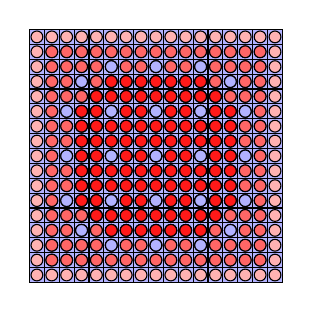
\begin{tikzpicture}[scale=0.15, every node/.style={scale=1}]
        \foreach \x in {0,1.26,...,20.16}
        \foreach \y in {0,1.26,...,20.16}
        \filldraw[xshift=\x cm, yshift=\y cm, fill=blue!30!white, 
        draw=black] (0, 0) rectangle (1.26,1.26) node[pos=.5] {};
        \foreach \x in {0,1.26,...,20.16}
        \foreach \y in {0,1.26,...,20.16}
        \filldraw[xshift=\x cm, yshift=\y cm, fill=red!30!white, draw=black] 
        (.63,.63) circle (.5) node[pos=.5] {};
        \foreach \x in {1.26,2.52,...,20.16}
        \foreach \y in {1.26,2.52,...,20.16}
        \filldraw[xshift=\x cm, yshift=\y cm, fill=red!60!white, draw=black] 
        (.63,.63) circle (.5) node[pos=.5] {};
        \foreach \x in {5*1.26,6*1.26,7*1.26,8*1.26,9*1.26,10*1.26,11*1.26}
        \foreach \y in {3*1.26,13*1.26}
        \filldraw[xshift=\x cm, yshift=\y cm, fill=red!90!white, draw=black] 
        (.63,.63) circle (.5) node[pos=.5] {};
        \foreach \x in 
        {4*1.26,5*1.26,6*1.26,7*1.26,8*1.26,9*1.26,10*1.26,11*1.26,12*1.26}
        \foreach \y in {4*1.26,12*1.26}
        \filldraw[xshift=\x cm, yshift=\y cm, fill=red!90!white, draw=black] 
        (.63,.63) circle (.5) node[pos=.5] {};
        \foreach \x in {3.78,5.04,...,16.38}
        \foreach \y in {6.3,7.56,...,15.04}
        \filldraw[xshift=\x cm, yshift=\y cm, fill=red!90!white, draw=black] 
        (.63,.63) circle (.5) node[pos=.5] {};
        \foreach \x in {5*1.26, 8*1.26, 11*1.26}
        \foreach \y in {2*1.26, 14*1.26}
        \filldraw[xshift=\x cm, yshift=\y cm, fill=blue!30!white, 
        draw=black] (.63,.63) circle (.5) node[pos=.5] {};
        \foreach \x in {3*1.26, 13*1.26}
        \foreach \y in {3*1.26, 13*1.26}
        \filldraw[xshift=\x cm, yshift=\y cm, fill=blue!30!white, 
        draw=black] (.63,.63) circle (.5) node[pos=.5] {};
        \foreach \x in {2*1.26, 5*1.26, 8*1.26, 11*1.26, 14*1.26}
        \foreach \y in {5*1.26, 8*1.26, 11*1.26}
        \filldraw[xshift=\x cm, yshift=\y cm, fill=blue!30!white, 
        draw=black] (.63,.63) circle (.5) node[pos=.5] {};
    \end{tikzpicture}
    \label{fig:MOX_config}
\end{figure}
\end{column}
\end{columns}
\end{frame}


\begin{frame}
\frametitle{2D C5G7}
\begin{figure}
\centering
\includegraphics[width = 0.9\textwidth]{figures/dmd_ospi_semilog_c5g7.pdf}
\end{figure}
\end{frame}

\section{Conclusion and Future Work}
\begin{frame}
\frametitle{Conclusion and Future Work}
\begin{block}{Conclusion}
\begin{enumerate}
\item 5x speedup for DMD-PM(n)
\item 5x-10x speedup for DMD-FPM(n)
\end{enumerate}
\end{block}
\begin{block}{ Future Work}
\begin{enumerate}
\item Acceleration of Monte Carlo Method 
\item Accurate Estimation of Eigenvalue for the flattened Power Method 
\end{enumerate}
\end{block}
\end{frame}  

\begin{frame}
\frametitle{Acknowledgement}
\begin{block}{Acknowledgement}
\begin{enumerate}
\item Alan Levin Department of Mechanical and Nuclear Engineering
\item Dr. Roberts
\item My Parents
\item Many Friends and colleagues: Richard, Dr. Mohammad Abdo,  Dr. Wenkai Fu, John, Rabab, Ye, Cheikh, Khalid, Dr. Luis Wonnell, Dipta
\end{enumerate}
\end{block}
\end{frame}

\beginbackup % begins the non-numbered slides

\end{document}
